\documentclass[twoside]{book}

% Packages required by doxygen
\usepackage{fixltx2e}
\usepackage{calc}
\usepackage{doxygen}
\usepackage[export]{adjustbox} % also loads graphicx
\usepackage{graphicx}
\usepackage[utf8]{inputenc}
\usepackage{makeidx}
\usepackage{multicol}
\usepackage{multirow}
\PassOptionsToPackage{warn}{textcomp}
\usepackage{textcomp}
\usepackage[nointegrals]{wasysym}
\usepackage[table]{xcolor}

% Font selection
\usepackage[T1]{fontenc}
\usepackage[scaled=.90]{helvet}
\usepackage{courier}
\usepackage{amssymb}
\usepackage{sectsty}
\renewcommand{\familydefault}{\sfdefault}
\allsectionsfont{%
  \fontseries{bc}\selectfont%
  \color{darkgray}%
}
\renewcommand{\DoxyLabelFont}{%
  \fontseries{bc}\selectfont%
  \color{darkgray}%
}
\newcommand{\+}{\discretionary{\mbox{\scriptsize$\hookleftarrow$}}{}{}}

% Page & text layout
\usepackage{geometry}
\geometry{%
  a4paper,%
  top=2.5cm,%
  bottom=2.5cm,%
  left=2.5cm,%
  right=2.5cm%
}
\tolerance=750
\hfuzz=15pt
\hbadness=750
\setlength{\emergencystretch}{15pt}
\setlength{\parindent}{0cm}
\setlength{\parskip}{3ex plus 2ex minus 2ex}
\makeatletter
\renewcommand{\paragraph}{%
  \@startsection{paragraph}{4}{0ex}{-1.0ex}{1.0ex}{%
    \normalfont\normalsize\bfseries\SS@parafont%
  }%
}
\renewcommand{\subparagraph}{%
  \@startsection{subparagraph}{5}{0ex}{-1.0ex}{1.0ex}{%
    \normalfont\normalsize\bfseries\SS@subparafont%
  }%
}
\makeatother

% Headers & footers
\usepackage{fancyhdr}
\pagestyle{fancyplain}
\fancyhead[LE]{\fancyplain{}{\bfseries\thepage}}
\fancyhead[CE]{\fancyplain{}{}}
\fancyhead[RE]{\fancyplain{}{\bfseries\leftmark}}
\fancyhead[LO]{\fancyplain{}{\bfseries\rightmark}}
\fancyhead[CO]{\fancyplain{}{}}
\fancyhead[RO]{\fancyplain{}{\bfseries\thepage}}
\fancyfoot[LE]{\fancyplain{}{}}
\fancyfoot[CE]{\fancyplain{}{}}
\fancyfoot[RE]{\fancyplain{}{\bfseries\scriptsize Generated by Doxygen }}
\fancyfoot[LO]{\fancyplain{}{\bfseries\scriptsize Generated by Doxygen }}
\fancyfoot[CO]{\fancyplain{}{}}
\fancyfoot[RO]{\fancyplain{}{}}
\renewcommand{\footrulewidth}{0.4pt}
\renewcommand{\chaptermark}[1]{%
  \markboth{#1}{}%
}
\renewcommand{\sectionmark}[1]{%
  \markright{\thesection\ #1}%
}

% Indices & bibliography
\usepackage{natbib}
\usepackage[titles]{tocloft}
\setcounter{tocdepth}{3}
\setcounter{secnumdepth}{5}
\makeindex

% Hyperlinks (required, but should be loaded last)
\usepackage{ifpdf}
\ifpdf
  \usepackage[pdftex,pagebackref=true]{hyperref}
\else
  \usepackage[ps2pdf,pagebackref=true]{hyperref}
\fi
\hypersetup{%
  colorlinks=true,%
  linkcolor=blue,%
  citecolor=blue,%
  unicode%
}

% Custom commands
\newcommand{\clearemptydoublepage}{%
  \newpage{\pagestyle{empty}\cleardoublepage}%
}

\usepackage{caption}
\captionsetup{labelsep=space,justification=centering,font={bf},singlelinecheck=off,skip=4pt,position=top}

%===== C O N T E N T S =====

\begin{document}

% Titlepage & ToC
\hypersetup{pageanchor=false,
             bookmarksnumbered=true,
             pdfencoding=unicode
            }
\pagenumbering{alph}
\begin{titlepage}
\vspace*{7cm}
\begin{center}%
{\Large Project Connect }\\
\vspace*{1cm}
{\large Generated by Doxygen 1.8.13}\\
\end{center}
\end{titlepage}
\clearemptydoublepage
\pagenumbering{roman}
\tableofcontents
\clearemptydoublepage
\pagenumbering{arabic}
\hypersetup{pageanchor=true}

%--- Begin generated contents ---
\chapter{Project\+\_\+connect}
\label{md__home_thomas_Documents_M2_Archi_logiciel_project_connect_README}
\Hypertarget{md__home_thomas_Documents_M2_Archi_logiciel_project_connect_README}
Based on M\+Q\+TT and QT Framework this projet contains all applications for gateway and sensor

I. \hyperlink{classGateway}{Gateway} Message router between the graphics application and the sensors

II. \hyperlink{classSensor}{Sensor} Air Quality Transmitting the quality of the air

II. \hyperlink{classSensor}{Sensor} Flame Detector/ Bar\+Graph Alert the graphic application of fire detection and receives the air quality to display

I\+II. \hyperlink{classSensor}{Sensor} Environnemental Transmitting pressure, temperature, and humidity 
\chapter{Hierarchical Index}
\section{Class Hierarchy}
This inheritance list is sorted roughly, but not completely, alphabetically\+:\begin{DoxyCompactList}
\item Q\+Object\begin{DoxyCompactList}
\item \contentsline{section}{Air\+Quality}{\pageref{classAirQuality}}{}
\item \contentsline{section}{Mqtt\+Handler}{\pageref{classMqttHandler}}{}
\begin{DoxyCompactList}
\item \contentsline{section}{Gateway}{\pageref{classGateway}}{}
\item \contentsline{section}{Mqtt\+Com}{\pageref{classMqttCom}}{}
\item \contentsline{section}{Mqtt\+Sensor}{\pageref{classMqttSensor}}{}
\item \contentsline{section}{Sensor}{\pageref{classSensor}}{}
\end{DoxyCompactList}
\item \contentsline{section}{Sensor}{\pageref{classSensor}}{}
\item \contentsline{section}{Sensor\+Gpio\+Data}{\pageref{classSensorGpioData}}{}
\item \contentsline{section}{Sensor\+Value}{\pageref{classSensorValue}}{}
\end{DoxyCompactList}
\end{DoxyCompactList}

\chapter{Class Index}
\section{Class List}
Here are the classes, structs, unions and interfaces with brief descriptions\+:\begin{DoxyCompactList}
\item\contentsline{section}{\hyperlink{classAirQuality}{Air\+Quality} }{\pageref{classAirQuality}}{}
\item\contentsline{section}{\hyperlink{classGateway}{Gateway} }{\pageref{classGateway}}{}
\item\contentsline{section}{\hyperlink{classMqttCom}{Mqtt\+Com} }{\pageref{classMqttCom}}{}
\item\contentsline{section}{\hyperlink{classMqttHandler}{Mqtt\+Handler} \\*The \hyperlink{classMqttHandler}{Mqtt\+Handler} class }{\pageref{classMqttHandler}}{}
\item\contentsline{section}{\hyperlink{classMqttSensor}{Mqtt\+Sensor} \\*The \hyperlink{classMqttSensor}{Mqtt\+Sensor} class }{\pageref{classMqttSensor}}{}
\item\contentsline{section}{\hyperlink{classSensor}{Sensor} \\*The \hyperlink{classSensor}{Sensor} class }{\pageref{classSensor}}{}
\item\contentsline{section}{\hyperlink{classSensorGpioData}{Sensor\+Gpio\+Data} \\*The Receive\+Data class }{\pageref{classSensorGpioData}}{}
\item\contentsline{section}{\hyperlink{classSensorValue}{Sensor\+Value} \\*The \hyperlink{classSensorValue}{Sensor\+Value} class }{\pageref{classSensorValue}}{}
\end{DoxyCompactList}

\chapter{File Index}
\section{File List}
Here is a list of all documented files with brief descriptions\+:\begin{DoxyCompactList}
\item\contentsline{section}{/home/thomas/\+Documents/\+M2/\+Archi\+\_\+logiciel/project\+\_\+connect/airquality/{\bfseries airquality.\+h} }{\pageref{airquality_8h}}{}
\item\contentsline{section}{/home/thomas/\+Documents/\+M2/\+Archi\+\_\+logiciel/project\+\_\+connect/airquality/{\bfseries mqttcom.\+h} }{\pageref{mqttcom_8h}}{}
\item\contentsline{section}{/home/thomas/\+Documents/\+M2/\+Archi\+\_\+logiciel/project\+\_\+connect/bme280/\hyperlink{MqttSensor_8cpp}{Mqtt\+Sensor.\+cpp} \\*A Document file }{\pageref{MqttSensor_8cpp}}{}
\item\contentsline{section}{/home/thomas/\+Documents/\+M2/\+Archi\+\_\+logiciel/project\+\_\+connect/bme280/\hyperlink{MqttSensor_8h}{Mqtt\+Sensor.\+h} \\*A Document file }{\pageref{MqttSensor_8h}}{}
\item\contentsline{section}{/home/thomas/\+Documents/\+M2/\+Archi\+\_\+logiciel/project\+\_\+connect/bme280/{\bfseries Sensor.\+h} }{\pageref{bme280_2Sensor_8h}}{}
\item\contentsline{section}{/home/thomas/\+Documents/\+M2/\+Archi\+\_\+logiciel/project\+\_\+connect/bme280/\hyperlink{SensorValue_8cpp}{Sensor\+Value.\+cpp} \\*A Document file }{\pageref{SensorValue_8cpp}}{}
\item\contentsline{section}{/home/thomas/\+Documents/\+M2/\+Archi\+\_\+logiciel/project\+\_\+connect/bme280/\hyperlink{SensorValue_8h}{Sensor\+Value.\+h} \\*A Document file }{\pageref{SensorValue_8h}}{}
\item\contentsline{section}{/home/thomas/\+Documents/\+M2/\+Archi\+\_\+logiciel/project\+\_\+connect/flame\+Graph/{\bfseries Sensor.\+h} }{\pageref{flameGraph_2Sensor_8h}}{}
\item\contentsline{section}{/home/thomas/\+Documents/\+M2/\+Archi\+\_\+logiciel/project\+\_\+connect/flame\+Graph/{\bfseries Sensor\+Gpio\+Data.\+h} }{\pageref{SensorGpioData_8h}}{}
\item\contentsline{section}{/home/thomas/\+Documents/\+M2/\+Archi\+\_\+logiciel/project\+\_\+connect/gateway/{\bfseries gateway.\+h} }{\pageref{gateway_8h}}{}
\item\contentsline{section}{/home/thomas/\+Documents/\+M2/\+Archi\+\_\+logiciel/project\+\_\+connect/mqtthandler/{\bfseries mqtthandler.\+h} }{\pageref{mqtthandler_8h}}{}
\end{DoxyCompactList}

\chapter{Class Documentation}
\hypertarget{classAirQuality}{}\section{Air\+Quality Class Reference}
\label{classAirQuality}\index{Air\+Quality@{Air\+Quality}}
Inheritance diagram for Air\+Quality\+:\begin{figure}[H]
\begin{center}
\leavevmode
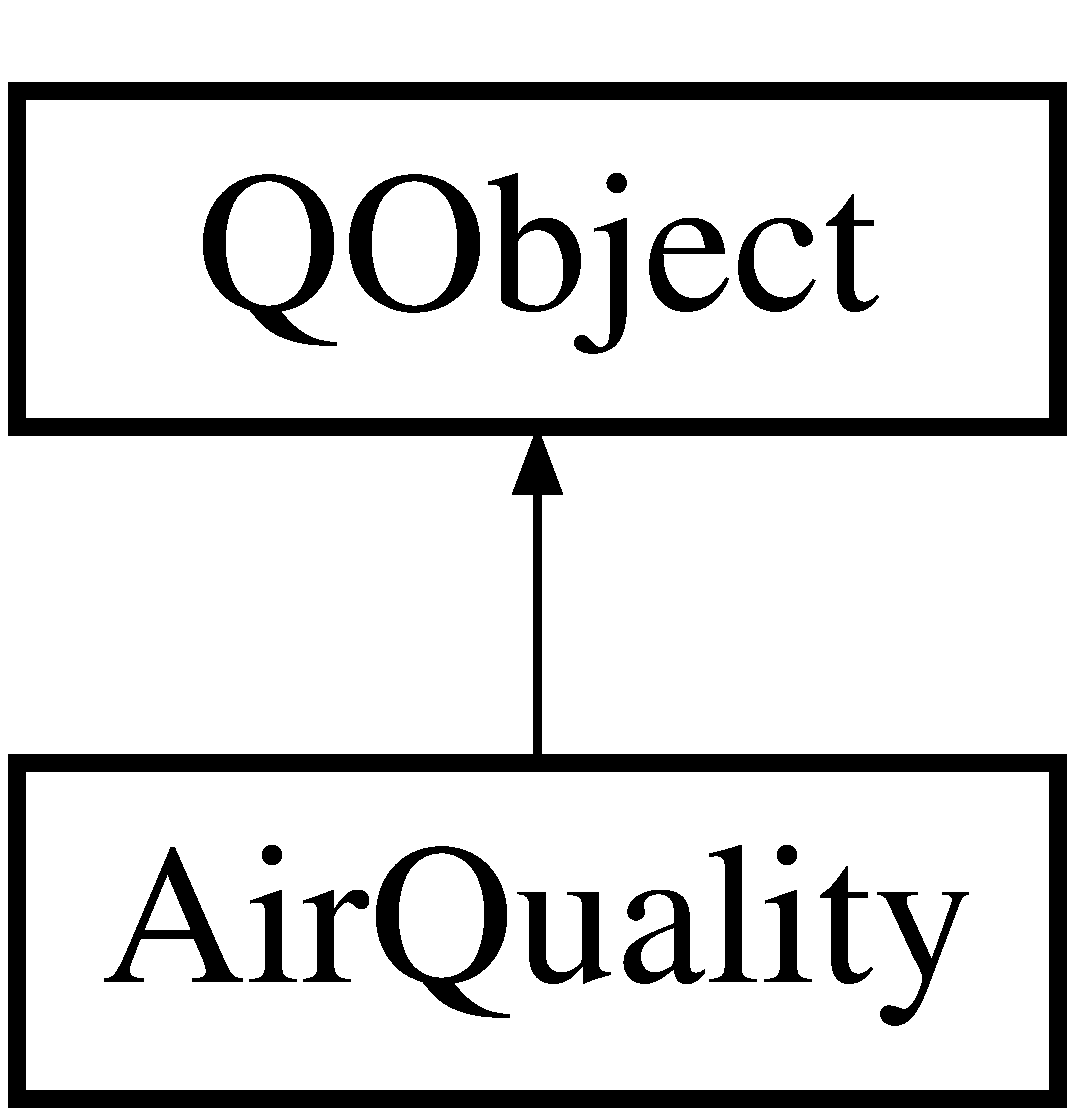
\includegraphics[height=2.000000cm]{classAirQuality}
\end{center}
\end{figure}
\subsection*{Public Slots}
\begin{DoxyCompactItemize}
\item 
\mbox{\Hypertarget{classAirQuality_a16c9cfb7cb19bc6eabbbede97f2cb125}\label{classAirQuality_a16c9cfb7cb19bc6eabbbede97f2cb125}} 
void {\bfseries read\+Sensor} ()
\item 
\mbox{\Hypertarget{classAirQuality_ac34f79a7f17b82dc19e584d3b5f0425e}\label{classAirQuality_ac34f79a7f17b82dc19e584d3b5f0425e}} 
void {\bfseries timer\+Slot} ()
\end{DoxyCompactItemize}
\subsection*{Signals}
\begin{DoxyCompactItemize}
\item 
\mbox{\Hypertarget{classAirQuality_a1109f52aee3643b1ef0bef0f3df5870f}\label{classAirQuality_a1109f52aee3643b1ef0bef0f3df5870f}} 
void {\bfseries on\+Data\+Sensor} (Q\+String topic, Q\+Json\+Object payload)
\end{DoxyCompactItemize}
\subsection*{Public Member Functions}
\begin{DoxyCompactItemize}
\item 
\mbox{\Hypertarget{classAirQuality_a780c19f099ebc69346ca85557372d7e3}\label{classAirQuality_a780c19f099ebc69346ca85557372d7e3}} 
Q\+String {\bfseries read\+Co2} ()
\item 
\mbox{\Hypertarget{classAirQuality_abf89a765a16eebf241db36cefeb82a7d}\label{classAirQuality_abf89a765a16eebf241db36cefeb82a7d}} 
Q\+String {\bfseries read\+Tvoc} ()
\end{DoxyCompactItemize}


The documentation for this class was generated from the following files\+:\begin{DoxyCompactItemize}
\item 
/home/thomas/\+Documents/\+M2/\+Archi\+\_\+logiciel/project\+\_\+connect/airquality/airquality.\+h\item 
/home/thomas/\+Documents/\+M2/\+Archi\+\_\+logiciel/project\+\_\+connect/airquality/airquality.\+cpp\end{DoxyCompactItemize}

\hypertarget{classGateway}{}\section{Gateway Class Reference}
\label{classGateway}\index{Gateway@{Gateway}}
Inheritance diagram for Gateway\+:\begin{figure}[H]
\begin{center}
\leavevmode
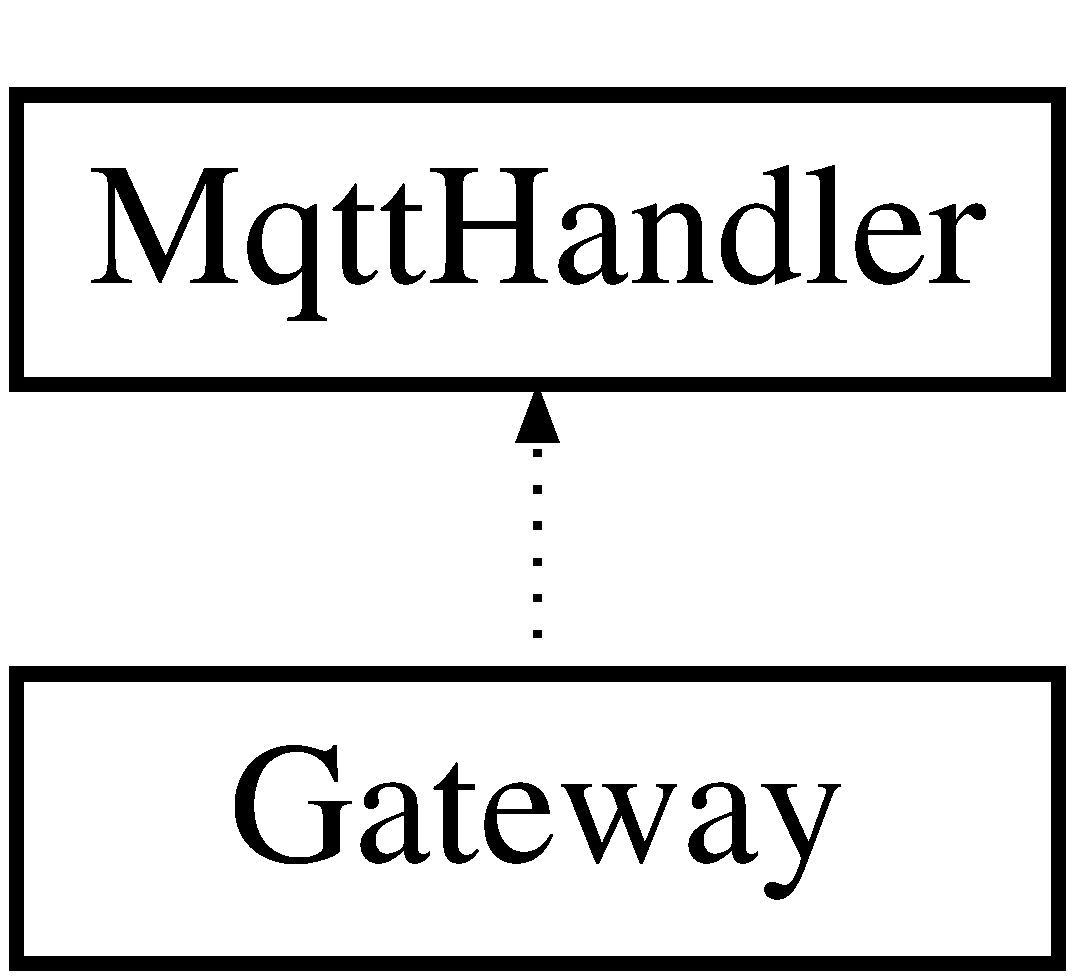
\includegraphics[height=2.000000cm]{classGateway}
\end{center}
\end{figure}
\subsection*{Public Slots}
\begin{DoxyCompactItemize}
\item 
\mbox{\Hypertarget{classGateway_ac01214063bf478d3b9ea55fd2bcfde5c}\label{classGateway_ac01214063bf478d3b9ea55fd2bcfde5c}} 
void {\bfseries on\+Message} (Q\+Mqtt\+Message message)
\end{DoxyCompactItemize}
\subsection*{Public Member Functions}
\begin{DoxyCompactItemize}
\item 
\mbox{\Hypertarget{classGateway_a8fe609498219f1284486b6f7b9b6abd5}\label{classGateway_a8fe609498219f1284486b6f7b9b6abd5}} 
{\bfseries Gateway} (Q\+String address, quint16 port, Q\+List$<$ Q\+String $>$ topic\+List)
\end{DoxyCompactItemize}


The documentation for this class was generated from the following files\+:\begin{DoxyCompactItemize}
\item 
/home/thomas/\+Documents/\+M2/\+Archi\+\_\+logiciel/project\+\_\+connect/gateway/gateway.\+h\item 
/home/thomas/\+Documents/\+M2/\+Archi\+\_\+logiciel/project\+\_\+connect/gateway/gateway.\+cpp\end{DoxyCompactItemize}

\hypertarget{classMqttCom}{}\section{Mqtt\+Com Class Reference}
\label{classMqttCom}\index{Mqtt\+Com@{Mqtt\+Com}}
Inheritance diagram for Mqtt\+Com\+:\begin{figure}[H]
\begin{center}
\leavevmode
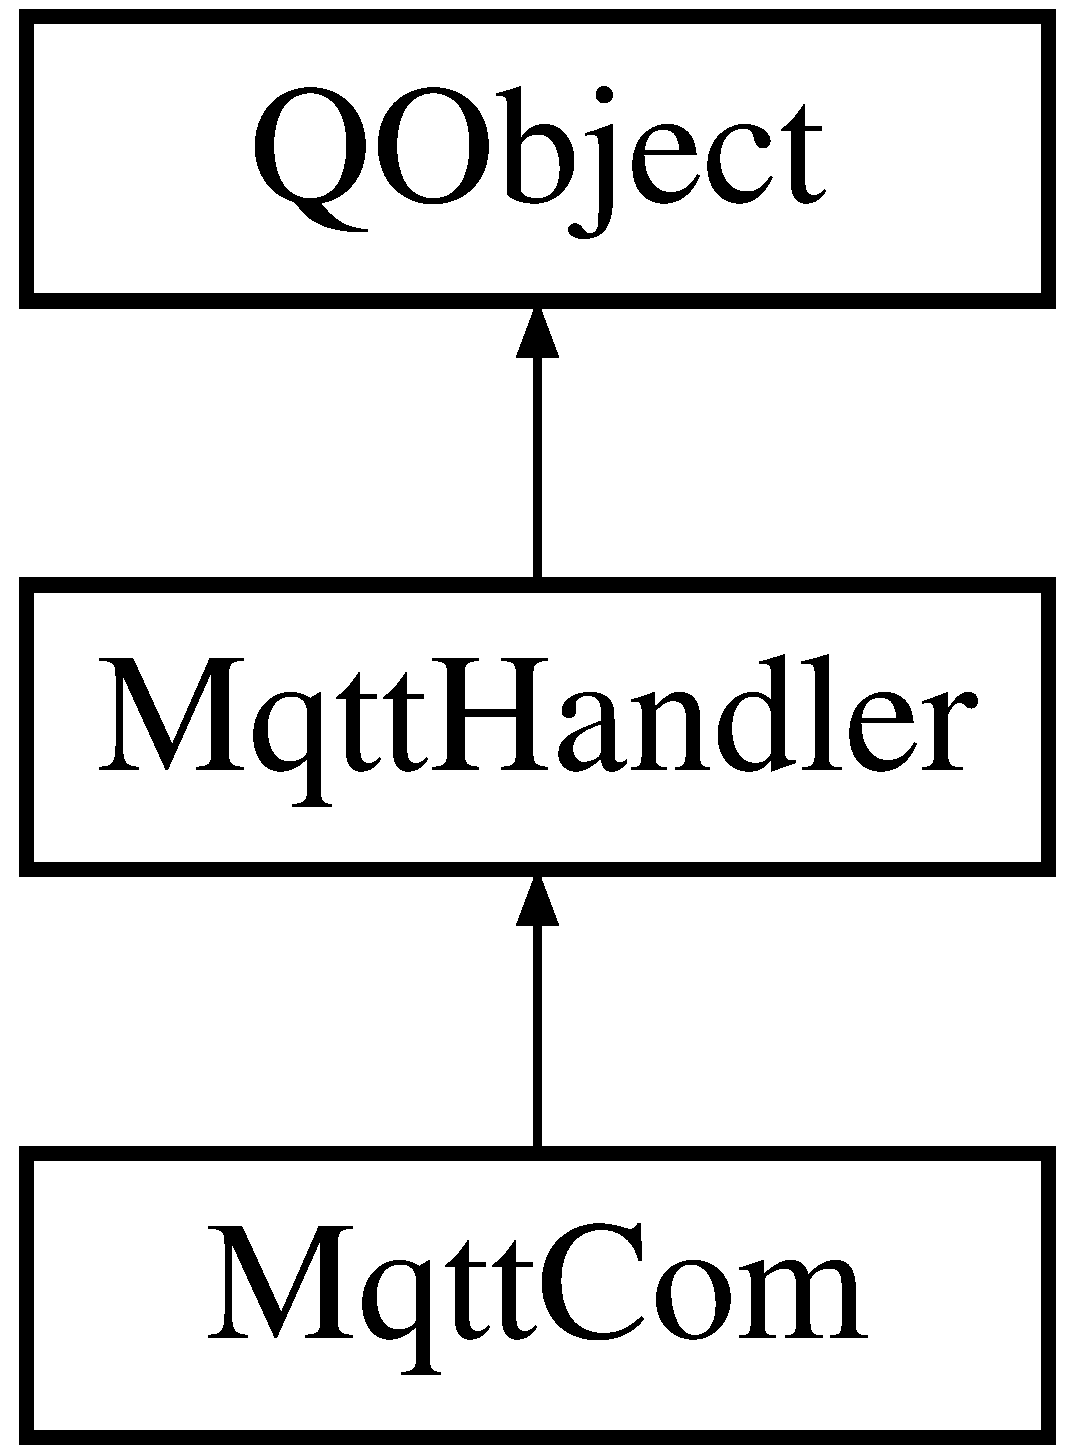
\includegraphics[height=3.000000cm]{classMqttCom}
\end{center}
\end{figure}
\subsection*{Public Slots}
\begin{DoxyCompactItemize}
\item 
\mbox{\Hypertarget{classMqttCom_aa7c8df5147b9906c3f6d50b65b9f828c}\label{classMqttCom_aa7c8df5147b9906c3f6d50b65b9f828c}} 
void {\bfseries on\+Message} (Q\+Mqtt\+Message message)
\item 
\mbox{\Hypertarget{classMqttCom_a2653bb72611cb7499d3e95e3a64556d6}\label{classMqttCom_a2653bb72611cb7499d3e95e3a64556d6}} 
void {\bfseries on\+Measure\+Sensor} (Q\+String topic, Q\+Json\+Object json\+Data)
\end{DoxyCompactItemize}
\subsection*{Public Member Functions}
\begin{DoxyCompactItemize}
\item 
\mbox{\Hypertarget{classMqttCom_a34917fc19aa7d9dfa67f647ed57e11bc}\label{classMqttCom_a34917fc19aa7d9dfa67f647ed57e11bc}} 
{\bfseries Mqtt\+Com} (Q\+String address, quint16 port, Q\+List$<$ Q\+String $>$ topic\+List)
\end{DoxyCompactItemize}
\subsection*{Additional Inherited Members}


The documentation for this class was generated from the following files\+:\begin{DoxyCompactItemize}
\item 
/home/thomas/\+Documents/\+M2/\+Archi\+\_\+logiciel/project\+\_\+connect/airquality/mqttcom.\+h\item 
/home/thomas/\+Documents/\+M2/\+Archi\+\_\+logiciel/project\+\_\+connect/airquality/mqttcom.\+cpp\end{DoxyCompactItemize}

\hypertarget{classMqttHandler}{}\section{Mqtt\+Handler Class Reference}
\label{classMqttHandler}\index{Mqtt\+Handler@{Mqtt\+Handler}}


The \hyperlink{classMqttHandler}{Mqtt\+Handler} class.  




{\ttfamily \#include $<$mqtthandler.\+h$>$}

Inheritance diagram for Mqtt\+Handler\+:\begin{figure}[H]
\begin{center}
\leavevmode
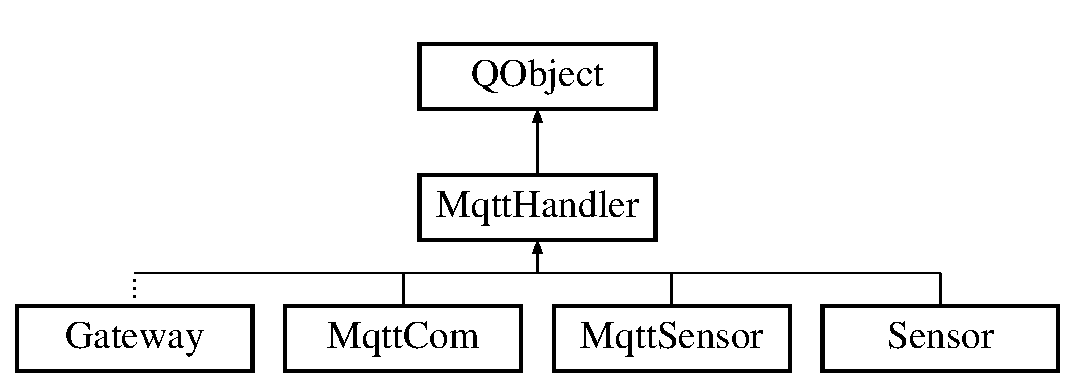
\includegraphics[height=3.000000cm]{classMqttHandler}
\end{center}
\end{figure}
\subsection*{Public Slots}
\begin{DoxyCompactItemize}
\item 
virtual void \hyperlink{classMqttHandler_acfaf00fbb740ea1c01c747c614a04c28}{on\+Message} (Q\+Mqtt\+Message message)
\begin{DoxyCompactList}\small\item\em on\+Message \end{DoxyCompactList}\end{DoxyCompactItemize}
\subsection*{Public Member Functions}
\begin{DoxyCompactItemize}
\item 
\hyperlink{classMqttHandler_a82b5c651c2777c831f186e6a9819bd50}{Mqtt\+Handler} (Q\+String \&address, quint16 port, Q\+List$<$ Q\+String $>$ topic\+List)
\begin{DoxyCompactList}\small\item\em \hyperlink{classMqttHandler}{Mqtt\+Handler}. \end{DoxyCompactList}\item 
\mbox{\Hypertarget{classMqttHandler_ad7c8c03663ca1139d9ad1954df76375e}\label{classMqttHandler_ad7c8c03663ca1139d9ad1954df76375e}} 
\hyperlink{classMqttHandler_ad7c8c03663ca1139d9ad1954df76375e}{$\sim$\+Mqtt\+Handler} ()
\begin{DoxyCompactList}\small\item\em Destroy the Mqtt Handler\+:\+: Mqtt Handler object. \end{DoxyCompactList}\item 
void \hyperlink{classMqttHandler_ac8d16d953468567ff9676e2bb71b9238}{publish\+Data} (Q\+String \&topic, Q\+Json\+Object \&json\+Data)
\begin{DoxyCompactList}\small\item\em publish\+Data \end{DoxyCompactList}\end{DoxyCompactItemize}
\subsection*{Public Attributes}
\begin{DoxyCompactItemize}
\item 
\mbox{\Hypertarget{classMqttHandler_a8d06cf85d6988c9c9129e170dda38a10}\label{classMqttHandler_a8d06cf85d6988c9c9129e170dda38a10}} 
Q\+Mqtt\+Client $\ast$ \hyperlink{classMqttHandler_a8d06cf85d6988c9c9129e170dda38a10}{m\+\_\+client}
\begin{DoxyCompactList}\small\item\em m\+\_\+client \end{DoxyCompactList}\end{DoxyCompactItemize}


\subsection{Detailed Description}
The \hyperlink{classMqttHandler}{Mqtt\+Handler} class. 

\subsection{Constructor \& Destructor Documentation}
\mbox{\Hypertarget{classMqttHandler_a82b5c651c2777c831f186e6a9819bd50}\label{classMqttHandler_a82b5c651c2777c831f186e6a9819bd50}} 
\index{Mqtt\+Handler@{Mqtt\+Handler}!Mqtt\+Handler@{Mqtt\+Handler}}
\index{Mqtt\+Handler@{Mqtt\+Handler}!Mqtt\+Handler@{Mqtt\+Handler}}
\subsubsection{\texorpdfstring{Mqtt\+Handler()}{MqttHandler()}}
{\footnotesize\ttfamily Mqtt\+Handler\+::\+Mqtt\+Handler (\begin{DoxyParamCaption}\item[{Q\+String \&}]{address,  }\item[{quint16}]{port,  }\item[{Q\+List$<$ Q\+String $>$}]{topic\+List }\end{DoxyParamCaption})}



\hyperlink{classMqttHandler}{Mqtt\+Handler}. 

Construct a new Mqtt Handler\+:\+: Mqtt Handler object.


\begin{DoxyParams}{Parameters}
{\em address} & \\
\hline
{\em port} & \\
\hline
{\em topic\+List} & \\
\hline
\end{DoxyParams}


\subsection{Member Function Documentation}
\mbox{\Hypertarget{classMqttHandler_acfaf00fbb740ea1c01c747c614a04c28}\label{classMqttHandler_acfaf00fbb740ea1c01c747c614a04c28}} 
\index{Mqtt\+Handler@{Mqtt\+Handler}!on\+Message@{on\+Message}}
\index{on\+Message@{on\+Message}!Mqtt\+Handler@{Mqtt\+Handler}}
\subsubsection{\texorpdfstring{on\+Message}{onMessage}}
{\footnotesize\ttfamily void Mqtt\+Handler\+::on\+Message (\begin{DoxyParamCaption}\item[{Q\+Mqtt\+Message}]{message }\end{DoxyParamCaption})\hspace{0.3cm}{\ttfamily [virtual]}, {\ttfamily [slot]}}



on\+Message 


\begin{DoxyParams}{Parameters}
{\em message} & \\
\hline
\end{DoxyParams}
\mbox{\Hypertarget{classMqttHandler_ac8d16d953468567ff9676e2bb71b9238}\label{classMqttHandler_ac8d16d953468567ff9676e2bb71b9238}} 
\index{Mqtt\+Handler@{Mqtt\+Handler}!publish\+Data@{publish\+Data}}
\index{publish\+Data@{publish\+Data}!Mqtt\+Handler@{Mqtt\+Handler}}
\subsubsection{\texorpdfstring{publish\+Data()}{publishData()}}
{\footnotesize\ttfamily void Mqtt\+Handler\+::publish\+Data (\begin{DoxyParamCaption}\item[{Q\+String \&}]{topic,  }\item[{Q\+Json\+Object \&}]{json\+Data }\end{DoxyParamCaption})}



publish\+Data 


\begin{DoxyParams}{Parameters}
{\em topic} & \\
\hline
{\em json\+Data} & \\
\hline
\end{DoxyParams}


The documentation for this class was generated from the following files\+:\begin{DoxyCompactItemize}
\item 
/home/thomas/\+Documents/\+M2/\+Archi\+\_\+logiciel/project\+\_\+connect/mqtthandler/mqtthandler.\+h\item 
/home/thomas/\+Documents/\+M2/\+Archi\+\_\+logiciel/project\+\_\+connect/mqtthandler/mqtthandler.\+cpp\end{DoxyCompactItemize}

\hypertarget{classMqttSensor}{}\section{Mqtt\+Sensor Class Reference}
\label{classMqttSensor}\index{Mqtt\+Sensor@{Mqtt\+Sensor}}


The \hyperlink{classMqttSensor}{Mqtt\+Sensor} class.  




{\ttfamily \#include $<$Mqtt\+Sensor.\+h$>$}

Inheritance diagram for Mqtt\+Sensor\+:\begin{figure}[H]
\begin{center}
\leavevmode
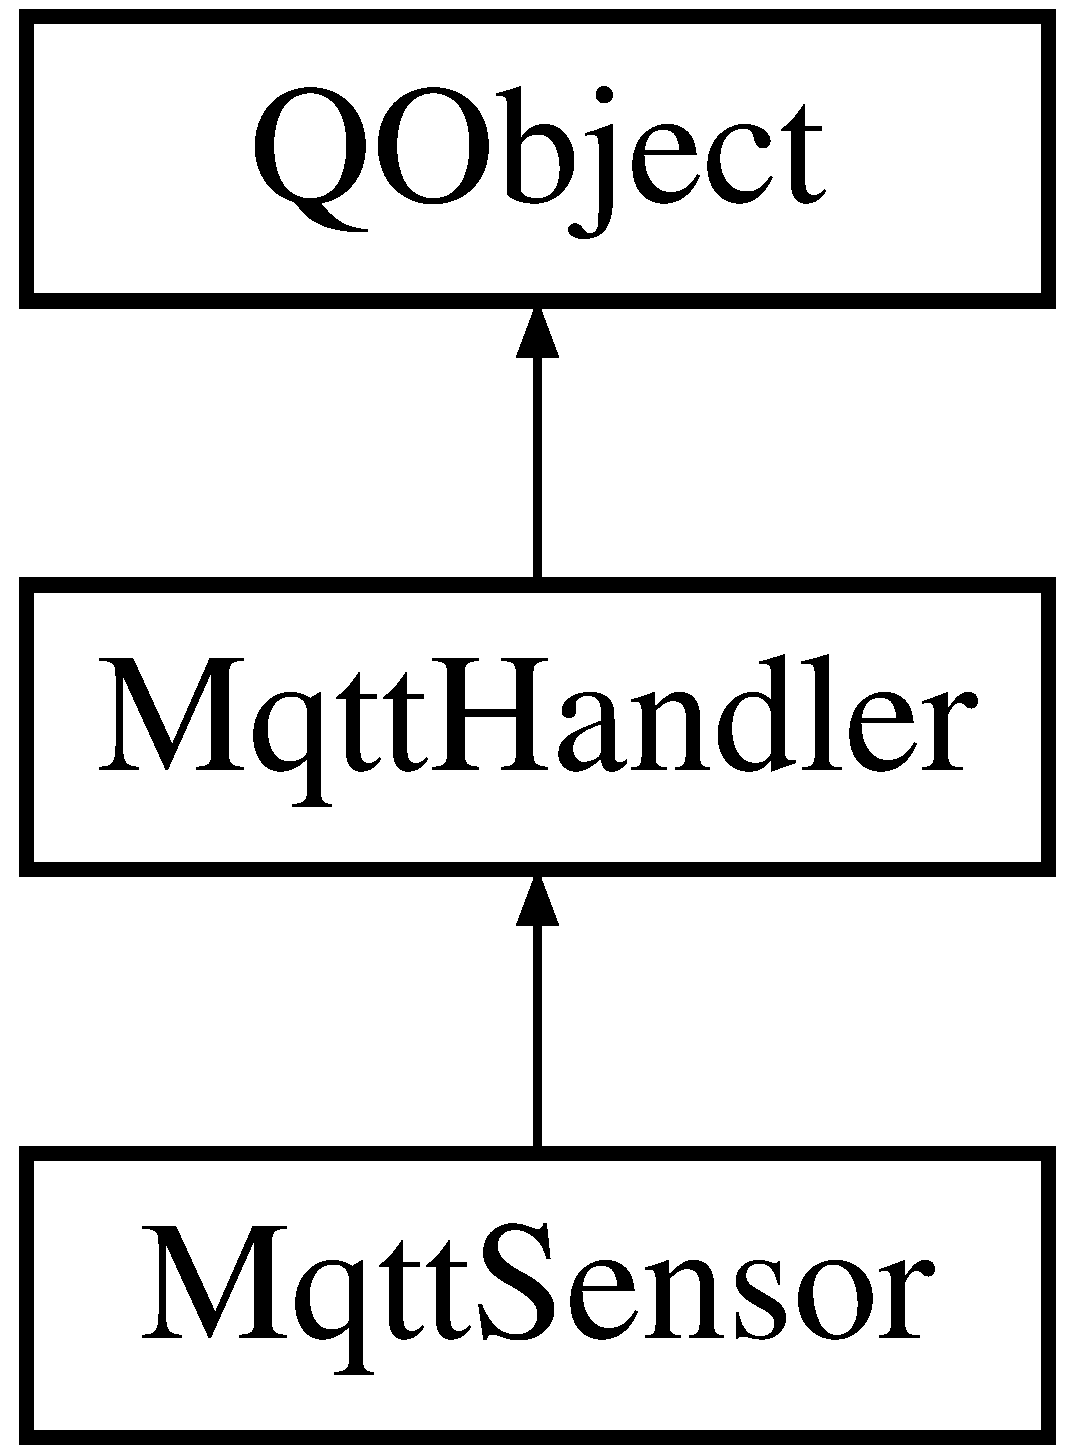
\includegraphics[height=3.000000cm]{classMqttSensor}
\end{center}
\end{figure}
\subsection*{Public Slots}
\begin{DoxyCompactItemize}
\item 
void \hyperlink{classMqttSensor_a5ced2fd35046b8306902358860cb3dce}{on\+Message} (Q\+Mqtt\+Message message) override
\begin{DoxyCompactList}\small\item\em \hyperlink{classMqttSensor_a5ced2fd35046b8306902358860cb3dce}{Mqtt\+Sensor\+::on\+Message}. \end{DoxyCompactList}\item 
void \hyperlink{classMqttSensor_a0e7aa8d83910d9481683b34bf3075321}{data\+Publish} (Q\+String Topic, Q\+Json\+Object data)
\begin{DoxyCompactList}\small\item\em Mqtt\+Sensor\+::data\+\_\+publish. \end{DoxyCompactList}\end{DoxyCompactItemize}
\subsection*{Public Member Functions}
\begin{DoxyCompactItemize}
\item 
\hyperlink{classMqttSensor_a2b6e93a22be073904ade69ce1af4e03f}{Mqtt\+Sensor} (Q\+String address, quint16 port, Q\+List$<$ Q\+String $>$ topic\+List)
\begin{DoxyCompactList}\small\item\em \hyperlink{classMqttSensor_a2b6e93a22be073904ade69ce1af4e03f}{Mqtt\+Sensor\+::\+Mqtt\+Sensor}. \end{DoxyCompactList}\end{DoxyCompactItemize}
\subsection*{Additional Inherited Members}


\subsection{Detailed Description}
The \hyperlink{classMqttSensor}{Mqtt\+Sensor} class. 

class allow connection of class 

\subsection{Constructor \& Destructor Documentation}
\mbox{\Hypertarget{classMqttSensor_a2b6e93a22be073904ade69ce1af4e03f}\label{classMqttSensor_a2b6e93a22be073904ade69ce1af4e03f}} 
\index{Mqtt\+Sensor@{Mqtt\+Sensor}!Mqtt\+Sensor@{Mqtt\+Sensor}}
\index{Mqtt\+Sensor@{Mqtt\+Sensor}!Mqtt\+Sensor@{Mqtt\+Sensor}}
\subsubsection{\texorpdfstring{Mqtt\+Sensor()}{MqttSensor()}}
{\footnotesize\ttfamily Mqtt\+Sensor\+::\+Mqtt\+Sensor (\begin{DoxyParamCaption}\item[{Q\+String}]{address,  }\item[{quint16}]{port,  }\item[{Q\+List$<$ Q\+String $>$}]{topic\+List }\end{DoxyParamCaption})}



\hyperlink{classMqttSensor_a2b6e93a22be073904ade69ce1af4e03f}{Mqtt\+Sensor\+::\+Mqtt\+Sensor}. 


\begin{DoxyParams}{Parameters}
{\em address} & address ip of gateway \\
\hline
{\em port} & 1883 \\
\hline
{\em topic\+List} & all topics using by the mqtt protocol \\
\hline
\end{DoxyParams}


\subsection{Member Function Documentation}
\mbox{\Hypertarget{classMqttSensor_a0e7aa8d83910d9481683b34bf3075321}\label{classMqttSensor_a0e7aa8d83910d9481683b34bf3075321}} 
\index{Mqtt\+Sensor@{Mqtt\+Sensor}!data\+Publish@{data\+Publish}}
\index{data\+Publish@{data\+Publish}!Mqtt\+Sensor@{Mqtt\+Sensor}}
\subsubsection{\texorpdfstring{data\+Publish}{dataPublish}}
{\footnotesize\ttfamily void Mqtt\+Sensor\+::data\+Publish (\begin{DoxyParamCaption}\item[{Q\+String}]{Topic,  }\item[{Q\+Json\+Object}]{data }\end{DoxyParamCaption})\hspace{0.3cm}{\ttfamily [slot]}}



Mqtt\+Sensor\+::data\+\_\+publish. 


\begin{DoxyParams}{Parameters}
{\em Topic} & \\
\hline
{\em data} & function transmit data via mqtt protocol \\
\hline
\end{DoxyParams}
\mbox{\Hypertarget{classMqttSensor_a5ced2fd35046b8306902358860cb3dce}\label{classMqttSensor_a5ced2fd35046b8306902358860cb3dce}} 
\index{Mqtt\+Sensor@{Mqtt\+Sensor}!on\+Message@{on\+Message}}
\index{on\+Message@{on\+Message}!Mqtt\+Sensor@{Mqtt\+Sensor}}
\subsubsection{\texorpdfstring{on\+Message}{onMessage}}
{\footnotesize\ttfamily void Mqtt\+Sensor\+::on\+Message (\begin{DoxyParamCaption}\item[{Q\+Mqtt\+Message}]{message }\end{DoxyParamCaption})\hspace{0.3cm}{\ttfamily [override]}, {\ttfamily [slot]}}



\hyperlink{classMqttSensor_a5ced2fd35046b8306902358860cb3dce}{Mqtt\+Sensor\+::on\+Message}. 


\begin{DoxyParams}{Parameters}
{\em message} & Function receiving data via mqtt protocol \\
\hline
\end{DoxyParams}


The documentation for this class was generated from the following files\+:\begin{DoxyCompactItemize}
\item 
/home/thomas/\+Documents/\+M2/\+Archi\+\_\+logiciel/project\+\_\+connect/bme280/\hyperlink{MqttSensor_8h}{Mqtt\+Sensor.\+h}\item 
/home/thomas/\+Documents/\+M2/\+Archi\+\_\+logiciel/project\+\_\+connect/bme280/\hyperlink{MqttSensor_8cpp}{Mqtt\+Sensor.\+cpp}\end{DoxyCompactItemize}

\hypertarget{classSensor}{}\section{Sensor Class Reference}
\label{classSensor}\index{Sensor@{Sensor}}


The \hyperlink{classSensor}{Sensor} class.  




{\ttfamily \#include $<$Sensor.\+h$>$}

Inheritance diagram for Sensor\+:\begin{figure}[H]
\begin{center}
\leavevmode
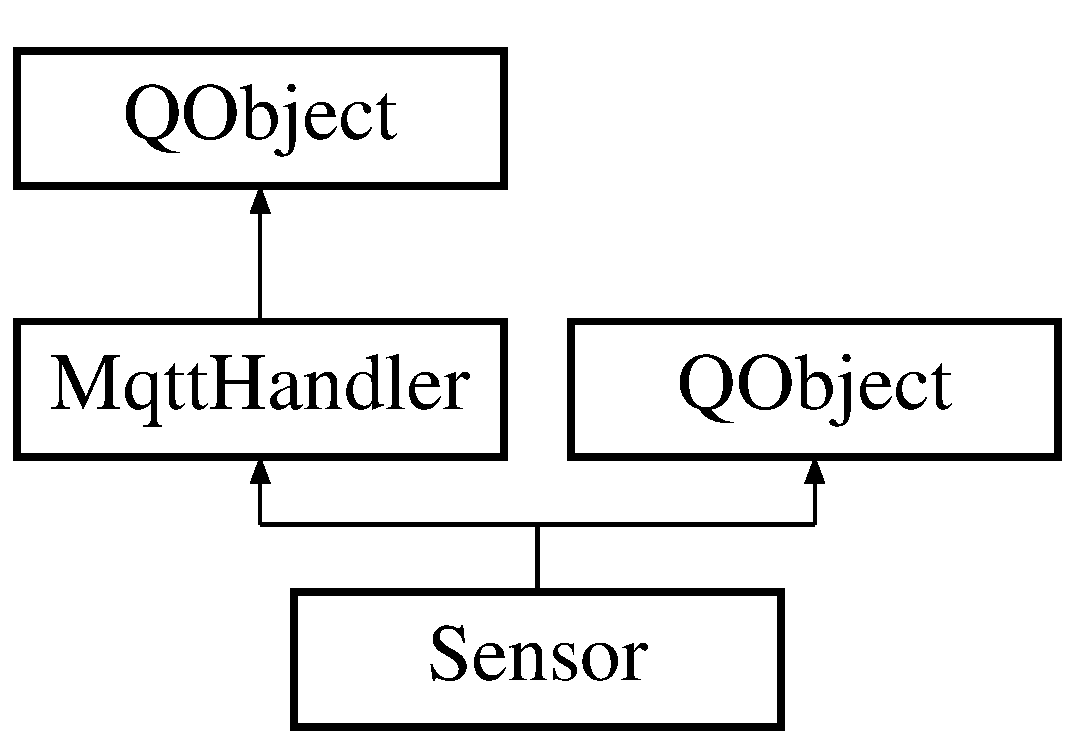
\includegraphics[height=3.000000cm]{classSensor}
\end{center}
\end{figure}
\subsection*{Public Slots}
\begin{DoxyCompactItemize}
\item 
void \hyperlink{classSensor_adead6577984a7d6b765897ba001ed176}{on\+Message} (Q\+Mqtt\+Message message) override
\begin{DoxyCompactList}\small\item\em \hyperlink{classSensor_adead6577984a7d6b765897ba001ed176}{Sensor\+::on\+Message} treatement of the message receive. \end{DoxyCompactList}\item 
void \hyperlink{classSensor_acace9ac9768e13174608c9e3649226f6}{Send\+Data} (Q\+String, Q\+Json\+Object)
\begin{DoxyCompactList}\small\item\em Send\+Data. \end{DoxyCompactList}\end{DoxyCompactItemize}
\subsection*{Public Member Functions}
\begin{DoxyCompactItemize}
\item 
\hyperlink{classSensor_a342d6d11ef572c8cba92cb76fb1a294b}{Sensor} ()
\begin{DoxyCompactList}\small\item\em \hyperlink{classSensor_a342d6d11ef572c8cba92cb76fb1a294b}{Sensor\+::\+Sensor} function collect the different class declaration of both class for connect call all the function for the sending of data. \end{DoxyCompactList}\item 
\mbox{\Hypertarget{classSensor_aee8c70e7ef05ce65e7ee33686b5d7db2}\label{classSensor_aee8c70e7ef05ce65e7ee33686b5d7db2}} 
\hyperlink{classSensor_aee8c70e7ef05ce65e7ee33686b5d7db2}{$\sim$\+Sensor} ()
\begin{DoxyCompactList}\small\item\em \hyperlink{classSensor_aee8c70e7ef05ce65e7ee33686b5d7db2}{Sensor\+::$\sim$\+Sensor}. \end{DoxyCompactList}\item 
\hyperlink{classSensor_a03d3f7e3089eaceba93b485c57e3b21d}{Sensor} (Q\+String address, quint16 port, Q\+List$<$ Q\+String $>$ topic\+List)
\begin{DoxyCompactList}\small\item\em Construct a new Inter Obj\+:\+: Inter Obj object this function make the connection beetween Receivedata and Comm\+Mqtt. \end{DoxyCompactList}\end{DoxyCompactItemize}
\subsection*{Additional Inherited Members}


\subsection{Detailed Description}
The \hyperlink{classSensor}{Sensor} class. 

connect the mqtt protocol and the data of sensor 

\subsection{Constructor \& Destructor Documentation}
\mbox{\Hypertarget{classSensor_a342d6d11ef572c8cba92cb76fb1a294b}\label{classSensor_a342d6d11ef572c8cba92cb76fb1a294b}} 
\index{Sensor@{Sensor}!Sensor@{Sensor}}
\index{Sensor@{Sensor}!Sensor@{Sensor}}
\subsubsection{\texorpdfstring{Sensor()}{Sensor()}\hspace{0.1cm}{\footnotesize\ttfamily [1/2]}}
{\footnotesize\ttfamily Sensor\+::\+Sensor (\begin{DoxyParamCaption}{ }\end{DoxyParamCaption})}



\hyperlink{classSensor_a342d6d11ef572c8cba92cb76fb1a294b}{Sensor\+::\+Sensor} function collect the different class declaration of both class for connect call all the function for the sending of data. 


\begin{DoxyParams}{Parameters}
{\em parent} & \\
\hline
\end{DoxyParams}
\mbox{\Hypertarget{classSensor_a03d3f7e3089eaceba93b485c57e3b21d}\label{classSensor_a03d3f7e3089eaceba93b485c57e3b21d}} 
\index{Sensor@{Sensor}!Sensor@{Sensor}}
\index{Sensor@{Sensor}!Sensor@{Sensor}}
\subsubsection{\texorpdfstring{Sensor()}{Sensor()}\hspace{0.1cm}{\footnotesize\ttfamily [2/2]}}
{\footnotesize\ttfamily Sensor\+::\+Sensor (\begin{DoxyParamCaption}\item[{Q\+String}]{address,  }\item[{quint16}]{port,  }\item[{Q\+List$<$ Q\+String $>$}]{topic\+List }\end{DoxyParamCaption})}



Construct a new Inter Obj\+:\+: Inter Obj object this function make the connection beetween Receivedata and Comm\+Mqtt. 


\begin{DoxyParams}{Parameters}
{\em parent} & \\
\hline
\end{DoxyParams}
object gpio chip 

\subsection{Member Function Documentation}
\mbox{\Hypertarget{classSensor_adead6577984a7d6b765897ba001ed176}\label{classSensor_adead6577984a7d6b765897ba001ed176}} 
\index{Sensor@{Sensor}!on\+Message@{on\+Message}}
\index{on\+Message@{on\+Message}!Sensor@{Sensor}}
\subsubsection{\texorpdfstring{on\+Message}{onMessage}}
{\footnotesize\ttfamily void Sensor\+::on\+Message (\begin{DoxyParamCaption}\item[{Q\+Mqtt\+Message}]{message }\end{DoxyParamCaption})\hspace{0.3cm}{\ttfamily [override]}, {\ttfamily [slot]}}



\hyperlink{classSensor_adead6577984a7d6b765897ba001ed176}{Sensor\+::on\+Message} treatement of the message receive. 


\begin{DoxyParams}{Parameters}
{\em message} & data receive from a pc \\
\hline
\end{DoxyParams}
\mbox{\Hypertarget{classSensor_acace9ac9768e13174608c9e3649226f6}\label{classSensor_acace9ac9768e13174608c9e3649226f6}} 
\index{Sensor@{Sensor}!Send\+Data@{Send\+Data}}
\index{Send\+Data@{Send\+Data}!Sensor@{Sensor}}
\subsubsection{\texorpdfstring{Send\+Data}{SendData}}
{\footnotesize\ttfamily void Sensor\+::\+Send\+Data (\begin{DoxyParamCaption}\item[{Q\+String}]{topic,  }\item[{Q\+Json\+Object}]{msg }\end{DoxyParamCaption})\hspace{0.3cm}{\ttfamily [slot]}}



Send\+Data. 

\hyperlink{classSensor_acace9ac9768e13174608c9e3649226f6}{Sensor\+::\+Send\+Data} Call the method publish of \hyperlink{classMqttHandler}{Mqtt\+Handler} to send data to the gateway.


\begin{DoxyParams}{Parameters}
{\em topic} & name of the topic where we want to send message \\
\hline
{\em msg} & data to send, in Q\+Json\+Object \\
\hline
\end{DoxyParams}


The documentation for this class was generated from the following files\+:\begin{DoxyCompactItemize}
\item 
/home/thomas/\+Documents/\+M2/\+Archi\+\_\+logiciel/project\+\_\+connect/bme280/Sensor.\+h\item 
/home/thomas/\+Documents/\+M2/\+Archi\+\_\+logiciel/project\+\_\+connect/bme280/Sensor.\+cpp\end{DoxyCompactItemize}

\hypertarget{classSensorGpioData}{}\section{Sensor\+Gpio\+Data Class Reference}
\label{classSensorGpioData}\index{Sensor\+Gpio\+Data@{Sensor\+Gpio\+Data}}


The Receive\+Data class.  




{\ttfamily \#include $<$Sensor\+Gpio\+Data.\+h$>$}

Inheritance diagram for Sensor\+Gpio\+Data\+:\begin{figure}[H]
\begin{center}
\leavevmode
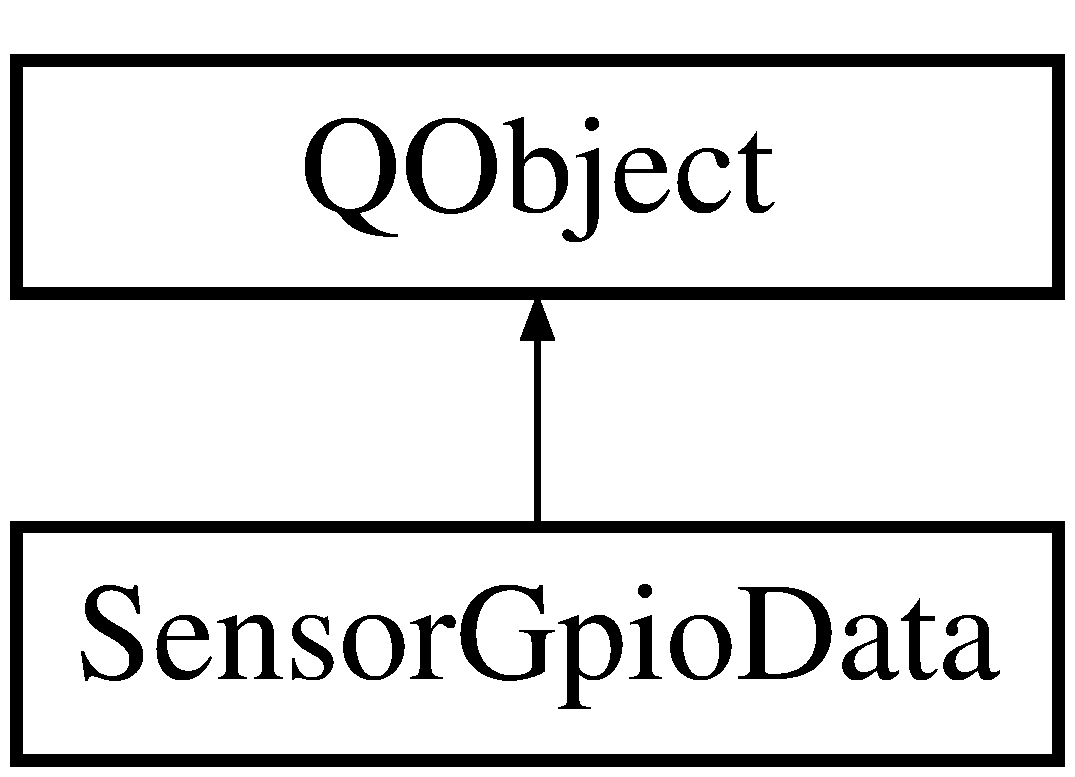
\includegraphics[height=2.000000cm]{classSensorGpioData}
\end{center}
\end{figure}
\subsection*{Public Slots}
\begin{DoxyCompactItemize}
\item 
\mbox{\Hypertarget{classSensorGpioData_a9978184c1074157ea029bcc4c305a937}\label{classSensorGpioData_a9978184c1074157ea029bcc4c305a937}} 
void \hyperlink{classSensorGpioData_a9978184c1074157ea029bcc4c305a937}{Gpio\+Event} ()
\begin{DoxyCompactList}\small\item\em Receive\+Data\+::timer\+Event this function are call when the timer is over, it take the bool flame pin value and send it. \end{DoxyCompactList}\end{DoxyCompactItemize}
\subsection*{Signals}
\begin{DoxyCompactItemize}
\item 
\mbox{\Hypertarget{classSensorGpioData_a627b8ceb7dff21b4e6ea4451191e109e}\label{classSensorGpioData_a627b8ceb7dff21b4e6ea4451191e109e}} 
void {\bfseries Data\+Gpio\+Ready} (Q\+String, Q\+Json\+Object)
\end{DoxyCompactItemize}
\subsection*{Public Member Functions}
\begin{DoxyCompactItemize}
\item 
\hyperlink{classSensorGpioData_a040047c46fd1f8f3f50aa17ed93c9360}{Sensor\+Gpio\+Data} ()
\begin{DoxyCompactList}\small\item\em Construct a new My Timer\+:\+: My Timer object. \end{DoxyCompactList}\end{DoxyCompactItemize}


\subsection{Detailed Description}
The Receive\+Data class. 

\subsection{Constructor \& Destructor Documentation}
\mbox{\Hypertarget{classSensorGpioData_a040047c46fd1f8f3f50aa17ed93c9360}\label{classSensorGpioData_a040047c46fd1f8f3f50aa17ed93c9360}} 
\index{Sensor\+Gpio\+Data@{Sensor\+Gpio\+Data}!Sensor\+Gpio\+Data@{Sensor\+Gpio\+Data}}
\index{Sensor\+Gpio\+Data@{Sensor\+Gpio\+Data}!Sensor\+Gpio\+Data@{Sensor\+Gpio\+Data}}
\subsubsection{\texorpdfstring{Sensor\+Gpio\+Data()}{SensorGpioData()}}
{\footnotesize\ttfamily Sensor\+Gpio\+Data\+::\+Sensor\+Gpio\+Data (\begin{DoxyParamCaption}{ }\end{DoxyParamCaption})}



Construct a new My Timer\+:\+: My Timer object. 


\begin{DoxyParams}{Parameters}
{\em parent} & \\
\hline
\end{DoxyParams}
object gpio chip 

The documentation for this class was generated from the following files\+:\begin{DoxyCompactItemize}
\item 
/home/thomas/\+Documents/\+M2/\+Archi\+\_\+logiciel/project\+\_\+connect/flame\+Graph/Sensor\+Gpio\+Data.\+h\item 
/home/thomas/\+Documents/\+M2/\+Archi\+\_\+logiciel/project\+\_\+connect/flame\+Graph/Sensor\+Gpio\+Data.\+cpp\end{DoxyCompactItemize}

\hypertarget{classSensorValue}{}\section{Sensor\+Value Class Reference}
\label{classSensorValue}\index{Sensor\+Value@{Sensor\+Value}}


The \hyperlink{classSensorValue}{Sensor\+Value} class.  




{\ttfamily \#include $<$Sensor\+Value.\+h$>$}

Inheritance diagram for Sensor\+Value\+:\begin{figure}[H]
\begin{center}
\leavevmode
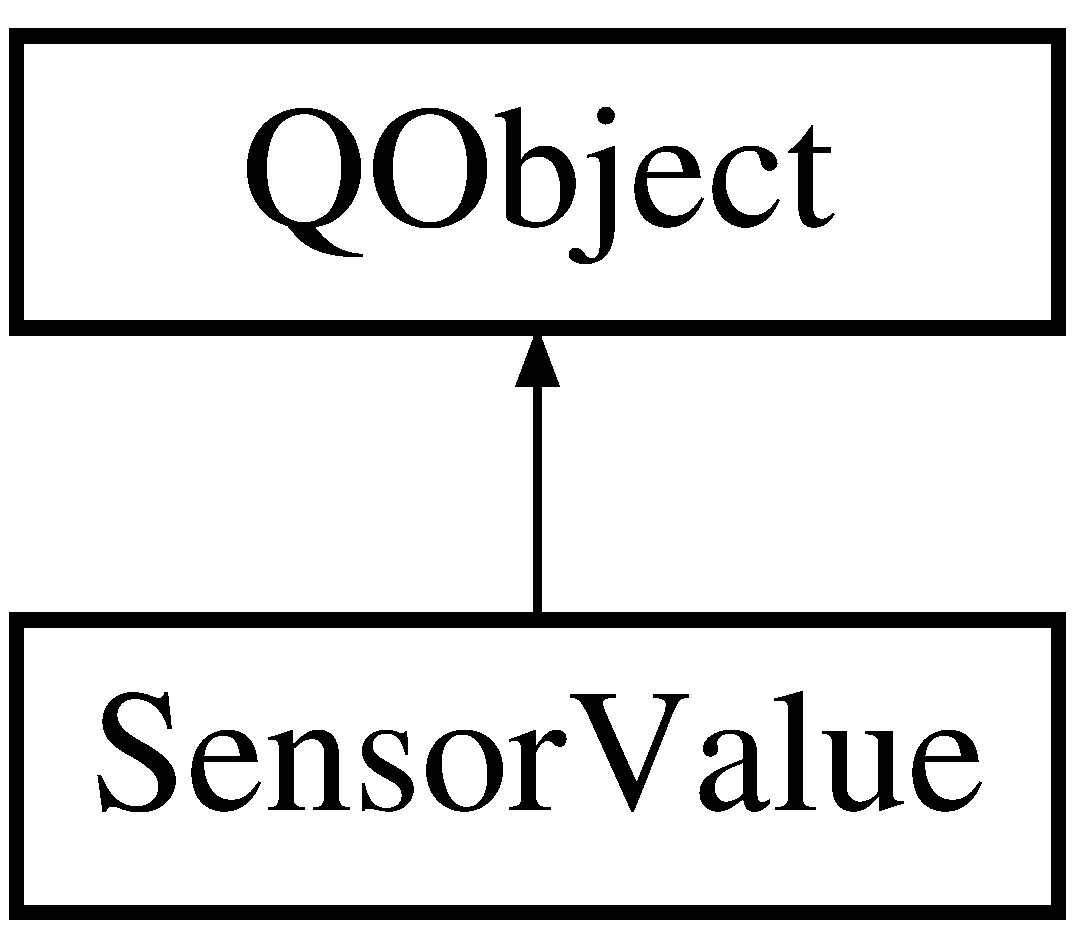
\includegraphics[height=2.000000cm]{classSensorValue}
\end{center}
\end{figure}
\subsection*{Public Slots}
\begin{DoxyCompactItemize}
\item 
void \hyperlink{classSensorValue_af24ff9ad2ade8fe703c4d67ae91fe3b5}{data\+Sensor} ()
\begin{DoxyCompactList}\small\item\em \hyperlink{classSensorValue_af24ff9ad2ade8fe703c4d67ae91fe3b5}{Sensor\+Value\+::data\+Sensor} read and convert data. \end{DoxyCompactList}\item 
void \hyperlink{classSensorValue_afa482d6ee6d1da567aad5c31f0118403}{send} (Q\+Json\+Object)
\begin{DoxyCompactList}\small\item\em \hyperlink{classSensorValue_afa482d6ee6d1da567aad5c31f0118403}{Sensor\+Value\+::send} send data with mqtt protocol the jobject of data sensor function will be send with this emit. \end{DoxyCompactList}\item 
double \hyperlink{classSensorValue_acf9b28e185a3f5c8c43bc409eb6d6723}{string\+To\+Value} (Q\+String)
\begin{DoxyCompactList}\small\item\em Sensor\+Value\+::stringtovalue function of conversion and reading in file the file contains the value of differents sensor. \end{DoxyCompactList}\item 
double \hyperlink{classSensorValue_a15d579b0938d2a8933f88563b108d150}{cast\+Value} (double, int)
\begin{DoxyCompactList}\small\item\em Sensor\+Value\+::cast\+\_\+value function allow choice the number after the comma. \end{DoxyCompactList}\end{DoxyCompactItemize}
\subsection*{Signals}
\begin{DoxyCompactItemize}
\item 
\mbox{\Hypertarget{classSensorValue_a3bc68cb111e1111f6f00495eac3c4cb4}\label{classSensorValue_a3bc68cb111e1111f6f00495eac3c4cb4}} 
void {\bfseries data\+Changed} (Q\+String, Q\+Json\+Object)
\end{DoxyCompactItemize}
\subsection*{Public Member Functions}
\begin{DoxyCompactItemize}
\item 
\hyperlink{classSensorValue_aed70ed5c17088bb9b420d9d63b9379bd}{Sensor\+Value} ()
\begin{DoxyCompactList}\small\item\em \hyperlink{classSensorValue_aed70ed5c17088bb9b420d9d63b9379bd}{Sensor\+Value\+::\+Sensor\+Value} function in interruption and called the function reading after a time define. \end{DoxyCompactList}\end{DoxyCompactItemize}
\subsection*{Public Attributes}
\begin{DoxyCompactItemize}
\item 
\mbox{\Hypertarget{classSensorValue_ac36ee5f0f2cd87e70ea805fd60642b9f}\label{classSensorValue_ac36ee5f0f2cd87e70ea805fd60642b9f}} 
Q\+File {\bfseries file}
\item 
\mbox{\Hypertarget{classSensorValue_a3a5569f5301c02e5519ef46c2ed42dfa}\label{classSensorValue_a3a5569f5301c02e5519ef46c2ed42dfa}} 
Q\+Text\+Stream {\bfseries flux}
\item 
\mbox{\Hypertarget{classSensorValue_a5d7d0853dfc7e6a107addcd5b0f367a9}\label{classSensorValue_a5d7d0853dfc7e6a107addcd5b0f367a9}} 
Q\+Timer $\ast$ {\bfseries timer}
\end{DoxyCompactItemize}


\subsection{Detailed Description}
The \hyperlink{classSensorValue}{Sensor\+Value} class. 

set up the reading and emit the data to mqtt protocol 

\subsection{Constructor \& Destructor Documentation}
\mbox{\Hypertarget{classSensorValue_aed70ed5c17088bb9b420d9d63b9379bd}\label{classSensorValue_aed70ed5c17088bb9b420d9d63b9379bd}} 
\index{Sensor\+Value@{Sensor\+Value}!Sensor\+Value@{Sensor\+Value}}
\index{Sensor\+Value@{Sensor\+Value}!Sensor\+Value@{Sensor\+Value}}
\subsubsection{\texorpdfstring{Sensor\+Value()}{SensorValue()}}
{\footnotesize\ttfamily Sensor\+Value\+::\+Sensor\+Value (\begin{DoxyParamCaption}{ }\end{DoxyParamCaption})}



\hyperlink{classSensorValue_aed70ed5c17088bb9b420d9d63b9379bd}{Sensor\+Value\+::\+Sensor\+Value} function in interruption and called the function reading after a time define. 

Q\+Object\+::connect connect timer with the function who will be called

\subsection{Member Function Documentation}
\mbox{\Hypertarget{classSensorValue_a15d579b0938d2a8933f88563b108d150}\label{classSensorValue_a15d579b0938d2a8933f88563b108d150}} 
\index{Sensor\+Value@{Sensor\+Value}!cast\+Value@{cast\+Value}}
\index{cast\+Value@{cast\+Value}!Sensor\+Value@{Sensor\+Value}}
\subsubsection{\texorpdfstring{cast\+Value}{castValue}}
{\footnotesize\ttfamily double Sensor\+Value\+::cast\+Value (\begin{DoxyParamCaption}\item[{double}]{valeur,  }\item[{int}]{n }\end{DoxyParamCaption})\hspace{0.3cm}{\ttfamily [slot]}}



Sensor\+Value\+::cast\+\_\+value function allow choice the number after the comma. 


\begin{DoxyParams}{Parameters}
{\em valeur} & contains the value who will be convert \\
\hline
{\em n} & number de digits after the comma \\
\hline
\end{DoxyParams}
\begin{DoxyReturn}{Returns}
return the value with a cast 
\end{DoxyReturn}
\mbox{\Hypertarget{classSensorValue_af24ff9ad2ade8fe703c4d67ae91fe3b5}\label{classSensorValue_af24ff9ad2ade8fe703c4d67ae91fe3b5}} 
\index{Sensor\+Value@{Sensor\+Value}!data\+Sensor@{data\+Sensor}}
\index{data\+Sensor@{data\+Sensor}!Sensor\+Value@{Sensor\+Value}}
\subsubsection{\texorpdfstring{data\+Sensor}{dataSensor}}
{\footnotesize\ttfamily void Sensor\+Value\+::data\+Sensor (\begin{DoxyParamCaption}{ }\end{DoxyParamCaption})\hspace{0.3cm}{\ttfamily [slot]}}



\hyperlink{classSensorValue_af24ff9ad2ade8fe703c4d67ae91fe3b5}{Sensor\+Value\+::data\+Sensor} read and convert data. 

add topics who will be use for the data sending \mbox{\Hypertarget{classSensorValue_afa482d6ee6d1da567aad5c31f0118403}\label{classSensorValue_afa482d6ee6d1da567aad5c31f0118403}} 
\index{Sensor\+Value@{Sensor\+Value}!send@{send}}
\index{send@{send}!Sensor\+Value@{Sensor\+Value}}
\subsubsection{\texorpdfstring{send}{send}}
{\footnotesize\ttfamily void Sensor\+Value\+::send (\begin{DoxyParamCaption}\item[{Q\+Json\+Object}]{data\+Sensor }\end{DoxyParamCaption})\hspace{0.3cm}{\ttfamily [slot]}}



\hyperlink{classSensorValue_afa482d6ee6d1da567aad5c31f0118403}{Sensor\+Value\+::send} send data with mqtt protocol the jobject of data sensor function will be send with this emit. 


\begin{DoxyParams}{Parameters}
{\em data\+\_\+sensor} & contains the data which must be send \\
\hline
\end{DoxyParams}
\mbox{\Hypertarget{classSensorValue_acf9b28e185a3f5c8c43bc409eb6d6723}\label{classSensorValue_acf9b28e185a3f5c8c43bc409eb6d6723}} 
\index{Sensor\+Value@{Sensor\+Value}!string\+To\+Value@{string\+To\+Value}}
\index{string\+To\+Value@{string\+To\+Value}!Sensor\+Value@{Sensor\+Value}}
\subsubsection{\texorpdfstring{string\+To\+Value}{stringToValue}}
{\footnotesize\ttfamily double Sensor\+Value\+::string\+To\+Value (\begin{DoxyParamCaption}\item[{Q\+String}]{path }\end{DoxyParamCaption})\hspace{0.3cm}{\ttfamily [slot]}}



Sensor\+Value\+::stringtovalue function of conversion and reading in file the file contains the value of differents sensor. 


\begin{DoxyParams}{Parameters}
{\em path} & contains the path which will be open \\
\hline
\end{DoxyParams}
\begin{DoxyReturn}{Returns}
the value contains in the file but in double type 
\end{DoxyReturn}


The documentation for this class was generated from the following files\+:\begin{DoxyCompactItemize}
\item 
/home/thomas/\+Documents/\+M2/\+Archi\+\_\+logiciel/project\+\_\+connect/bme280/\hyperlink{SensorValue_8h}{Sensor\+Value.\+h}\item 
/home/thomas/\+Documents/\+M2/\+Archi\+\_\+logiciel/project\+\_\+connect/bme280/\hyperlink{SensorValue_8cpp}{Sensor\+Value.\+cpp}\end{DoxyCompactItemize}

\chapter{File Documentation}
\hypertarget{MqttSensor_8cpp}{}\section{/home/thomas/\+Documents/\+M2/\+Archi\+\_\+logiciel/project\+\_\+connect/bme280/\+Mqtt\+Sensor.cpp File Reference}
\label{MqttSensor_8cpp}\index{/home/thomas/\+Documents/\+M2/\+Archi\+\_\+logiciel/project\+\_\+connect/bme280/\+Mqtt\+Sensor.\+cpp@{/home/thomas/\+Documents/\+M2/\+Archi\+\_\+logiciel/project\+\_\+connect/bme280/\+Mqtt\+Sensor.\+cpp}}


A Document file.  


{\ttfamily \#include \char`\"{}Mqtt\+Sensor.\+h\char`\"{}}\newline


\subsection{Detailed Description}
A Document file. 

\begin{DoxyAuthor}{Author}
Eric Rebillon (\href{mailto:eric.rebillon@ynov.com}{\tt eric.\+rebillon@ynov.\+com}) 
\end{DoxyAuthor}

\hypertarget{MqttSensor_8h}{}\section{/home/thomas/\+Documents/\+M2/\+Archi\+\_\+logiciel/project\+\_\+connect/bme280/\+Mqtt\+Sensor.h File Reference}
\label{MqttSensor_8h}\index{/home/thomas/\+Documents/\+M2/\+Archi\+\_\+logiciel/project\+\_\+connect/bme280/\+Mqtt\+Sensor.\+h@{/home/thomas/\+Documents/\+M2/\+Archi\+\_\+logiciel/project\+\_\+connect/bme280/\+Mqtt\+Sensor.\+h}}


A Document file.  


{\ttfamily \#include $<$Q\+List$>$}\newline
{\ttfamily \#include \char`\"{}mqtthandler.\+h\char`\"{}}\newline
\subsection*{Classes}
\begin{DoxyCompactItemize}
\item 
class \hyperlink{classMqttSensor}{Mqtt\+Sensor}
\begin{DoxyCompactList}\small\item\em The \hyperlink{classMqttSensor}{Mqtt\+Sensor} class. \end{DoxyCompactList}\end{DoxyCompactItemize}


\subsection{Detailed Description}
A Document file. 

\begin{DoxyAuthor}{Author}
Eric Rebillon (\href{mailto:eric.rebillon@ynov.com}{\tt eric.\+rebillon@ynov.\+com}) 
\end{DoxyAuthor}

\hypertarget{SensorValue_8cpp}{}\section{/home/thomas/\+Documents/\+M2/\+Archi\+\_\+logiciel/project\+\_\+connect/bme280/\+Sensor\+Value.cpp File Reference}
\label{SensorValue_8cpp}\index{/home/thomas/\+Documents/\+M2/\+Archi\+\_\+logiciel/project\+\_\+connect/bme280/\+Sensor\+Value.\+cpp@{/home/thomas/\+Documents/\+M2/\+Archi\+\_\+logiciel/project\+\_\+connect/bme280/\+Sensor\+Value.\+cpp}}


A Document file.  


{\ttfamily \#include \char`\"{}Sensor\+Value.\+h\char`\"{}}\newline


\subsection{Detailed Description}
A Document file. 

\begin{DoxyAuthor}{Author}
Eric Rebillon (\href{mailto:eric.rebillon@ynov.com}{\tt eric.\+rebillon@ynov.\+com}) 
\end{DoxyAuthor}

\hypertarget{SensorValue_8h}{}\section{/home/thomas/\+Documents/\+M2/\+Archi\+\_\+logiciel/project\+\_\+connect/bme280/\+Sensor\+Value.h File Reference}
\label{SensorValue_8h}\index{/home/thomas/\+Documents/\+M2/\+Archi\+\_\+logiciel/project\+\_\+connect/bme280/\+Sensor\+Value.\+h@{/home/thomas/\+Documents/\+M2/\+Archi\+\_\+logiciel/project\+\_\+connect/bme280/\+Sensor\+Value.\+h}}


A Document file.  


{\ttfamily \#include $<$Q\+File$>$}\newline
{\ttfamily \#include $<$Q\+Text\+Stream$>$}\newline
{\ttfamily \#include $<$Q\+String$>$}\newline
{\ttfamily \#include $<$Q\+Event$>$}\newline
{\ttfamily \#include $<$Q\+Timer$>$}\newline
{\ttfamily \#include $<$Q\+List$>$}\newline
{\ttfamily \#include $<$Q\+Debug$>$}\newline
{\ttfamily \#include $<$Q\+Json\+Object$>$}\newline
{\ttfamily \#include $<$Qt\+Math$>$}\newline
\subsection*{Classes}
\begin{DoxyCompactItemize}
\item 
class \hyperlink{classSensorValue}{Sensor\+Value}
\begin{DoxyCompactList}\small\item\em The \hyperlink{classSensorValue}{Sensor\+Value} class. \end{DoxyCompactList}\end{DoxyCompactItemize}
\subsection*{Macros}
\begin{DoxyCompactItemize}
\item 
\mbox{\Hypertarget{SensorValue_8h_aadfd306b31b445b9c008835a73790ef5}\label{SensorValue_8h_aadfd306b31b445b9c008835a73790ef5}} 
\#define {\bfseries P\+A\+T\+H\+\_\+\+T\+E\+M\+P\+E\+R\+A\+T\+U\+RE}~\char`\"{}/sys/bus/iio/devices/iio\textbackslash{}\+:device0/in\+\_\+temp\+\_\+input\char`\"{}
\item 
\mbox{\Hypertarget{SensorValue_8h_a352f1b064ffbcae68c91afd3ce27849d}\label{SensorValue_8h_a352f1b064ffbcae68c91afd3ce27849d}} 
\#define {\bfseries P\+A\+T\+H\+\_\+\+P\+R\+E\+S\+S\+I\+U\+RE}~\char`\"{}/sys/bus/iio/devices/iio\textbackslash{}\+:device0/in\+\_\+pressure\+\_\+input\char`\"{}
\item 
\mbox{\Hypertarget{SensorValue_8h_af35fc6e0cfbc2b765d9e496edccd8712}\label{SensorValue_8h_af35fc6e0cfbc2b765d9e496edccd8712}} 
\#define {\bfseries P\+A\+T\+H\+\_\+\+H\+U\+M\+I\+D\+I\+TY}~\char`\"{}/sys/bus/iio/devices/iio\textbackslash{}\+:device0/in\+\_\+humidityrelative\+\_\+input\char`\"{}
\item 
\mbox{\Hypertarget{SensorValue_8h_a1600b831de36293ba266ea4e148e838b}\label{SensorValue_8h_a1600b831de36293ba266ea4e148e838b}} 
\#define {\bfseries P\+A\+T\+H\+\_\+\+T\+E\+ST}~\char`\"{}/home/eric/Master1/workspace/Cpp\+\_\+project\+\_\+archi\+\_\+logicielle/fichier\+\_\+sim\+\_\+bme\+\_\+280.\+txt\char`\"{}
\item 
\mbox{\Hypertarget{SensorValue_8h_aef5816f45c406cf7d1c533418760cf2d}\label{SensorValue_8h_aef5816f45c406cf7d1c533418760cf2d}} 
\#define {\bfseries T\+O\+P\+I\+C\+\_\+\+T\+E\+M\+P\+E\+R\+A\+T\+U\+RE}~\char`\"{}/sensor/temperature\char`\"{}
\item 
\mbox{\Hypertarget{SensorValue_8h_ad30a27859ffa87adf31e6d39c1cc8bfe}\label{SensorValue_8h_ad30a27859ffa87adf31e6d39c1cc8bfe}} 
\#define {\bfseries T\+O\+P\+I\+C\+\_\+\+H\+U\+M\+I\+D\+I\+TY}~\char`\"{}/sensor/humidity\char`\"{}
\item 
\mbox{\Hypertarget{SensorValue_8h_a22bd07c32b8455e1ac1303bba3fe9de8}\label{SensorValue_8h_a22bd07c32b8455e1ac1303bba3fe9de8}} 
\#define {\bfseries T\+O\+P\+I\+C\+\_\+\+P\+R\+E\+S\+S\+I\+U\+RE}~\char`\"{}/sensor/pressure\char`\"{}
\item 
\mbox{\Hypertarget{SensorValue_8h_a76427053c362a0352c4985f74926482a}\label{SensorValue_8h_a76427053c362a0352c4985f74926482a}} 
\#define {\bfseries T\+O\+P\+I\+C\+\_\+\+E\+N\+V\+I\+R\+O\+N\+M\+E\+NT}~\char`\"{}/sensor/environment\char`\"{}
\item 
\mbox{\Hypertarget{SensorValue_8h_aef0259154abc7fdda6de05232a6a584f}\label{SensorValue_8h_aef0259154abc7fdda6de05232a6a584f}} 
\#define {\bfseries T\+M\+P\+\_\+\+T\+I\+M\+ER}~3000
\end{DoxyCompactItemize}


\subsection{Detailed Description}
A Document file. 

\begin{DoxyAuthor}{Author}
Eric Rebillon (\href{mailto:eric.rebillon@ynov.com}{\tt eric.\+rebillon@ynov.\+com}) 
\end{DoxyAuthor}

%--- End generated contents ---

% Index
\backmatter
\newpage
\phantomsection
\clearemptydoublepage
\addcontentsline{toc}{chapter}{Index}
\printindex

\end{document}
